\chapter{Automatic Verification of Refactored Code}
\label{chap:verification}

%  Approx 8-10 pages

% This chapter presents the second innovation: automated equivalence proofs
% without user annotations.

In the strictest sense, refactoring is defined as a behavior-preserving code
transformation. In practice, refactoring is only valuable if it preserves the
original program's behaviour. In Rust, where ownership and lifetimes enforce
strict invariants, the mere fact that refactored code compiles does not
guarantee equivalence. Additionally, because REM performs complex,
compiler-guided repairs as part of its extraction process
\cite{AdventureOfALifetime}, there is an increased risk of introducing subtle
changes in program behaviour. Subtle shifts in aliasing or lifetime structure
can produce programs that pass the compiler yet diverge semantically from their
originals. For high-assurance domains, this risk is unacceptable: automated
tools must not only generate compiling code but also provide evidence that
transformations are correct.

This chapoter introduces a novel verification pipeline that extends REM with
automatic, annotation-free proofs of equivalence between original and refactored
code. Our approach combines existing formal methods toolchains - CHARON
\footnote{More information accessible from their GitHub, \url{https://github.com/AeneasVerif/charon}}, which
translates Rust into an ownership-explicit intermediate from, and AENEAS
\footnote{More information accessible from their GitHub, \url{https://github.com/AeneasVerif/aeneas}}, which
then generates Coq code equivalent to the original Rust source through a pure
$\lambda$-calculus based intermediary. This Coq code can then be used
to formally prove that the refactored code is equivalent to the original.
The result is an end-to-end system in which the Extract $\rightarrow$ Repair
cyle is followed by a Verify phase, discharging proofs in seconds with no
additional burden on the developer. By embedding verification directly into the
refactoring process, we move beyond compilation success to true semantic
assurance, bridging the gap between theory and practical developer tools.

\section{Motivation: Why Verification is Essential}
\label{sec:motivation_verification}

Despite decades of work on automated refactoring, developers continue to show
reluctance to adopt such tools in practice. Empirical studies indicate that even
simple, “safe” refactorings such as renaming are frequently performed manually,
as programmers prefer to trust their own edits over opaque tool behaviour
\cite{OneThousandOneStories-SoftwareRefactoring}. This gap stems from usability
and, more fundamentally, from trust: if a refactoring tool cannot convincingly
guarantee that semantics are preserved, developers are unwilling to rely on it
for non-trivial code transformations.

The challenge is particularly acute in Rust. Compared to languages like Java or
C\#, where refactorings operate largely at the syntactic or type level, Rust's
ownership and lifetime system makes every transformation potentially semantic.
Prior work shows that Extract Method in Rust is not merely ``cut and paste'' but
requires compiler-guided repairs such as introducing lifetime parameters,
reifying control flow, and inferring ownership modes
\cite{AdventureOfALifetime}. Crucially, the final step to the original REM
algorithm involves a series of non-trivial lifetime adjustments, guided by
\verb|rustc|, to ensure that the extracted code satisfies the borrow checker.
These repairs enable REM to succeed where na\"ive tools fail, but they also
heighten the risk of unintended behavioural changes. A transformation that
compiles may nonetheless shift aliasing patterns, extend or shorten lifetimes,
or alter when resources are released — all of which are semantically observable
in Rust.

Traditional quality controls such as testing do not fill this gap. Tests, even
when comprehensive, explore only a small subset of possible inputs and
interleavings. In safety or performance critical domains, developers cannot
afford to accept the residual risk that untested paths diverge after a
refactoring. Verification, by contrast, offers a principled way to resolve the
trust deficit: it can establish - on a program by program basis - that for all
inputs respecting the refactored function's preconditioned, that the refactored
program is equivalent to the orginal. By integrating verification directly into
REM's pipeline, we address not only the technical challenge of making complex
extractions compile, but also the socio-technical challenge of making developers
confident that such transformations are behaviour-preserving.

\newpage
\section{Overview of the Verification Pipeline}
\label{verification pipeline}

\begin{wrapfigure}{tr}{0.5\textwidth} % r = right, width = half page
  \centering
  \vspace{\baselineskip}
  \vspace{\baselineskip}
  \vspace{\baselineskip}

  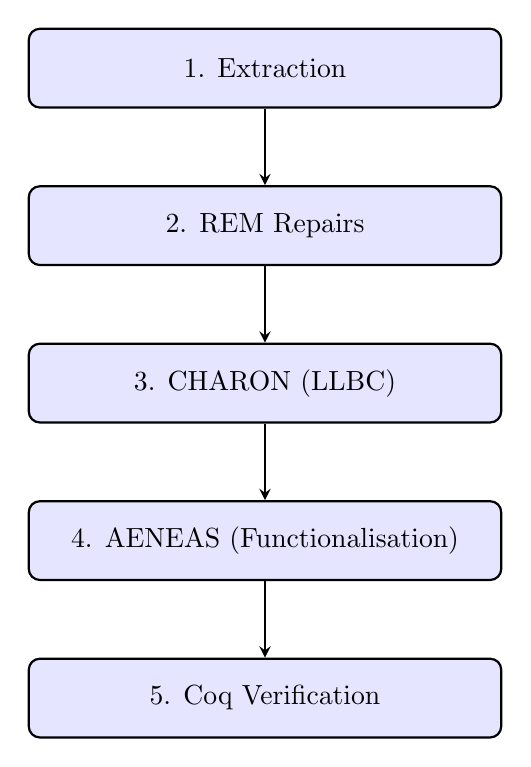
\begin{tikzpicture}[node distance=2cm, >=stealth, thick]
    % Nodes
    \node[draw, rounded corners, fill=blue!10, minimum width=6cm, minimum height=1cm] (extract) {1. Extraction};
    \node[draw, rounded corners, fill=blue!10, minimum width=6cm, minimum height=1cm, below of=extract] (rem) {2. REM Repairs};
    \node[draw, rounded corners, fill=blue!10, minimum width=6cm, minimum height=1cm, below of=rem] (charon) {3. CHARON (LLBC)};
    \node[draw, rounded corners, fill=blue!10, minimum width=6cm, minimum height=1cm, below of=charon] (aeneas) {4. AENEAS (Functionalisation)};
    \node[draw, rounded corners, fill=blue!10, minimum width=6cm, minimum
    height=1cm, below of=aeneas] (coq) {5. Coq Verification};

    % Arrows
    \draw[->] (extract) -- (rem);
    \draw[->] (rem) -- (charon);
    \draw[->] (charon) -- (aeneas);
    \draw[->] (aeneas) -- (coq);
  \end{tikzpicture}
  \caption{Overview of the verification pipeline: from source code extraction to proof of observational equivalence in Coq.}
  \label{fig:verification_pipeline}
\end{wrapfigure}

The verification pipeline augments REM's extract-and-repair workflow with an
automatic equivalence check. Its design is guided by two principles: (1)
verification must require no additional annotations or input from the developer,
and (2) it must complete quickly enough to fit into interactive IDE workflows.
To achieve this, the pipeline translates both the original program $P$ and the
refactored program $P'$ into progressively more structured semantic
representations, culminating in a machine-checked proof of observational
equivalence.

At a high level, the pipeline consists of five stages: \textbf{Extraction},
\textbf{REM repairs}, \textbf{CHARON translation}, \textbf{AENEAS
functionalisation}, and \textbf{Coq verification}. Each stage builds on the
previous one, gradually exposing the semantics of the refactored code while
preserving a clear correspondence to the original. Figure
~\ref{fig:verification_pipeline} provides an overview of the entire process.

\subsection{Extraction}

% Diagrams:
% Either a simple pre an post refactoring code snippet,
% Or a side by side of an example that needs nothing more than copy and paste,
% and a more complex one that needs repairs.

At the first stage, the user identifies a region of code to extract into a new
function. This can be done through REM's CLI, however, the VSCode extension
provides a much more user-friendly interface. The user highlights the code to be
extracted and invokes the extraction command. This step mirrors the mechanics of
traditional Extract Method refactorings: a block is lifted out of its enclosing
function, and a corresponding call is inserted in its place. At this point the
transformation is syntactic and only sometimes results in valid Rust. The below shows both cases:
\begin{itemize}
    \item The first is a simple extraction that requires no further repairs.
    Strict typing makes this a trivial case, and REM would not be called.
    \item The second is a more complex extraction that requires REM's repair
    phase to ensure the refactored code compiles. It is adapted from a real
    commit in \verb|GitOxide|\footnote{\url{https://github.com/GitoxideLabs/gitoxide/commit/c0786717c4979810002365a68d31abbf21d90f2d}},
    and was also used in ``Borrowing Without Sorrowing'' \cite{BorrowingWithoutSorrowing}.
    Note how the extraction algorithm has failed to find the lifetime parameter
    \verb|'a|, and added an unnecessary borrow of \verb|SectionID|. In this
    instance, REM would be called to fix the (non-compiling) code.
\end{itemize}

\begin{figure}[h]
\centering
\begin{subfigure}{0.45\linewidth}
  \inputminted[fontsize=\footnotesize, frame=none, linenos=false, breaklines=true, breakanywhere=true]{rust}{3_Chapter3/simple_original.rs}
  \caption{Simple function before extraction}
\end{subfigure}
\hfill
\begin{subfigure}{0.45\linewidth}
  \inputminted[fontsize=\footnotesize, frame=none, linenos=false, breaklines=true, breakanywhere=true]{rust}{3_Chapter3/simple_extracted.rs}
  \caption{Simple function after extraction}
\end{subfigure}

\vspace{1em}

\begin{subfigure}{0.45\linewidth}
  \inputminted[fontsize=\footnotesize, frame=none, linenos=false, breaklines=true, breakanywhere=true]{rust}{3_Chapter3/complex_original.rs}
  \caption{GitOxide function with manual extraction. See appendix \ref{sec:appendix_3} for details}
\end{subfigure}
\hfill
\begin{subfigure}{0.45\linewidth}
  \inputminted[fontsize=\footnotesize, frame=none, linenos=false, breaklines=true, breakanywhere=true]{rust}{3_Chapter3/complex_extracted.rs}
  \caption{GitOxide function with automated extraction}
  \label{content:bad_gitoxide_extraction}
\end{subfigure}

\caption{Two extraction examples: a trivial case (top) and a complex, failed case from real-world code (bottom).}
\label{fig:extraction_examples}
\end{figure}

\subsection{REM}

As seen in the above examples, a na\"ive extraction is often not going to
compile. Free variables, non-local control flow and lifetimes make the extracted
fragment ill-typed. the purpose of REM is to repair these issues automatically,
producing a valid Rust program $P'$ while preserving the intent of the original
code. At a high level, REM applies three classes of fixes:

\begin{enumerate}[label=(\roman*)]
    \item Reifying non-local control flow into a small result enum.
    \item Inferring ownership for free variables (by value, \verb|&T|, or
    \verb|&mut T|) and,
    \item Adjusting lifetime parameters in an iterative manner, guided by
    \verb|rustc| until the borrow checker is satisfied.
\end{enumerate}

These steps transform a purely syntactic extraction into a valid program $P'$
that is much closer to what a developer would have written by hand.

\subsubsection*{Example: Simple Case}

In the toy example, extraction is trivial. REM observes that both \verb|x| and
\verb|y| can be moved by valuie into the new function, so the inferred signature
is simply:

\begin{minted}[linenos,breaklines, frame=none, fontsize=\small]{rust}
fn add(x: i32, y: i32) -> i32
\end{minted}

No further repairs are needed. This illustrates the best case: REM's analysis
immediately determines that the signature is valid Rust and human readable.

\subsubsection*{Example: Real World Case}

By contrast, in the \verb|extract_include_path| example
(\ref{content:bad_gitoxide_extraction}), naiive extraction fails. The plugin
incorrectly infers that the loop variable \verb|id| must be borrowed
(\verb|&SectionID|), and entirely misses the lifetime parameter \verb|<'a>|,
required to properly scope our mutable references to \verb|File| and
\verb|Vec<path>| throughout the entire function.

REM corrects this in several ways:
\begin{enumerate}
    \item It detects that \verb|id| is consumed at the call site, so ownership
    can be transferred rather than borrowed.
    \item It generalises lifetime parameters across both \verb|File<'a>| and
    \verb|Vec<Path<'a>>| to ensure consistent scoping.
    \item It replays \verb|cargo check| until no lifetime mismatches remain.
\end{enumerate}

The resulting signature is significantly more natural (in this case it is
identical to the manual extraction).

\begin{minted}[linenos,breaklines, frame=none, fontsize=\small]{rust}
fn extract_include_path<'a>(
    target_config: &mut File<'a>,
    include_paths: &mut Vec<Path<'a>>,
    id: SectionId)
\end{minted}

The shift from \verb|&SectionId| to \verb|SectionId| demonstrates REM's key
contribution: making semantically appropriate ownership decisions automatically,
while still producing code that compiles under Rust's strict type system.

% TODO if I end up writing an incrementally compiling version of CHARON, add
% that information here.
\subsection{CHARON}
\label{subsec:charon}

The first stage of our verification pipeline is translation from Rust into a
lower-level, verification-friendly form. This role is performed by
\textbf{CHARON}, a Rust to LLBC (Low-Level Borrow Calculus) translator. CHARON
accepts Rust source code (or more precisely, its compiler intermediate
representation MIR) \footnote{Even more precisely, the tool itself accepts Rust
code, but its initial steps rely on a complex interaction with \texttt{rustc} to
acquire the MIR}. CHARON's main task is to extract complex semantic information
from \verb|rustc| and produce a machine readable output containing said
information.

CHARON performs several non-trivial transformations:
\begin{description}[leftmargin=!,labelwidth=2cm]
  \item[Structured control flow.] MIR is a control-flow graph with arbitrary
  \texttt{goto}s; CHARON reconstructs this into structured \texttt{if},
  \texttt{match}, and \texttt{loop} constructs, or preserves the raw form with
  the \texttt{--ullbc} option.
  \item[Trait and type resolution.] Explicitly records how trait bounds are
  proven, normalises default methods, and can transform associated types into
  explicit parameters (\texttt{--remove-associated-types}).
  \item[Lifetime handling.] Hides the distinction between early- and late-bound
  variables and makes implied bounds explicit, simplifying reasoning about
  generic functions. \item[Closures and vtables.] Represented as ordinary
  structs implementing the relevant
  \texttt{Fn*} traits, making them accessible to later verification steps.
  \item[Noise reduction.] Options such as \texttt{--hide-marker-traits} remove
  built-in traits (\texttt{Sized}, \texttt{Send}, etc.) that would otherwise
  clutter the output.
\end{description}

The result is a cleaned, semantically faithful program in LLBC form. Unlike raw
MIR, which is compiler-oriented, LLBC is designed for verification: ownership
and borrowing are represented directly, trait resolution is explicit, and
control flow is structured. A sample program and small portion of its MIR are
shown below. However, the output of CHARON is not designed for human
readability, and even the tiny program in Figure \ref{fig:charon_translation}
produces over 140,000 characters of LLBC. This (very verbose) explicitness is
what enables the subsequent translation into pure functional code for
verification.

\begin{figure}[ht]
  \centering
  \begin{minipage}[t]{0.45\linewidth}
    \inputminted[linenos, breaklines, frame=none, fontsize=\footnotesize]{rust}{3_Chapter3/CHARON_example/rust.rs}
    \vfill
    \caption*{Rust source}
  \end{minipage}
  \hfill
  \begin{minipage}[t]{0.45\linewidth}
    \inputminted[linenos, breaklines, frame=none, fontsize=\footnotesize]{text}{3_Chapter3/CHARON_example/mir.txt}
    \vfill
    \caption*{Excerpt of MIR (\texttt{rustc})}
  \end{minipage}
  \caption{Illustration of CHARON's role. While only Rust and MIR are shown here, CHARON translates the MIR into LLBC}
  \label{fig:charon_translation}
\end{figure}

\subsection{AENEAS}

With the program translated into LLBC by CHARON, the next stage of the pipeline
is handled by \textbf{AENEAS}. AENEAS takes the borrow- and lifetime–explicit
LLBC and translates it into a \emph{purely functional form}, stripping away
low-level memory operations while preserving the program's semantics. This
functionalisation step is what makes the program suitable for downstream
reasoning in Coq: instead of reasoning about references and loans, we can reason
about values and functions. Currently AENEAS supports translation into
\emph{Coq, Lean, HOL4}, and \emph{F*}.

In practice, AENEAS acts as the bridge between compiler-level detail and
proof-level abstraction. CHARON ensures that all the complexities of lifetimes,
loads, and trait resolution are made explicit; AENEAS then packages these into a
form where correctness properties can be stated and proved without touching the
borrow checker or the stack/heap. For our pipeline, this is the point where Rust
code ``stops being Rust'' and becomes a functional program whose equivalence can
be checked in Coq.

The central insight behind AENEAS is that Rust's ownership discipline makes much of low-level memory reasoning unnecessary.

\subsection{Coq}
% Potentially include a small paragraph here explaining what Coq is, for the uninitiated.

AENEAS translates the LLBC into a purely functional form, in this case Coq. The
final stage of the pipeline is thus to join the two Coq files ($P_{coq}$ and
$P'_{coq}$) with all of the auxiliary information needed to automatically verify
equivalence between the original and refactored Rust programs.

\subsubsection*{What is Coq?}
Coq is an interactive theorem prover and proof assistant built on a dependently
typed functional language. It allows developers to define mathematical objects,
programs, and logical propositions, and to construct machine-checked proofs
about them. Every proof is validated by Coq's small, trusted kernel, giving very
high assurance of correctness. Coq has a long history of use in large-scale
verification projects—such as CompCert (a verified C compiler) and formally
verified operating systems—making it a natural fit for reasoning about the
safety and correctness of Rust programs.

\subsubsection*{Why Coq?}
Coq was selected over alternatives such as HOL4, Lean, or F* for three main reasons:
\begin{description}[leftmargin=!,labelwidth=2.5cm]
    \item[Mature ecosystem] Decades of development have produced robust tooling, extensive libraries, and a stable kernel.
    \item[Direct integration] AENEAS already targets Coq, whereas HOL4 and Lean would require substantial new backends for compatibility.
    \item[Automation] Coq's tactic language and SMT integrations allow many routine proofs—such as equivalence checks—to be discharged automatically.
\end{description}

Lean and HOL4 both provide highly expressive logics, but at the cost of
significant engineering effort to integrate with AENEAS. F* is closer in spirit
to AENEAS, but the platform is less mature and would duplicate existing
functionality. Coq therefore offers the best combination of maturity,
automation, and direct compatibility with our pipeline.

\subsubsection*{Verification Examples}

To make the Coq stage of the pipeline concrete, we present two examples that
have followed the entire process from Rust source through to Coq. Together, they
illustrate both the best-case scenario and the additional complexity involved in
real-world refactorings.

Before looking at the translations themselves, it is worth noting the supporting
infrastructure. AENEAS generates not just the Coq files for individual
functions, but also a small project scaffold. The \texttt{Primitives.v} file
defines the Coq representations of Rust's core datatypes (\texttt{i32},
\texttt{Vec}, \texttt{Option}, etc.), providing a foundation on which the
translations depend. The \texttt{\_CoqProject} file ties the entire build
together, specifying load paths and dependencies so that the project can be
automatically compiled and checked consistently.

\begin{figure}[h]
  \centering
  \begin{minipage}{0.45\linewidth}
    \inputminted[linenos, breaklines, frame=none, fontsize=\footnotesize]{coq}{3_Chapter3/COQ_example/simple.v}
    \caption*{Simple example: original translation}
  \end{minipage}\hfill
  \begin{minipage}{0.45\linewidth}
    \inputminted[linenos, breaklines, frame=none, fontsize=\footnotesize]{coq}{3_Chapter3/COQ_example/simple_ref.v}
    \caption*{Simple example: refactored translation}
  \end{minipage}
  \caption{Coq translations for the simple example.}
  \label{fig:coq_simple}
\end{figure}

Alongside these translations, the verifyer produces the \texttt{EquivCheck.v}
file. This module instantiates both the original and refactored definitions and
generates an equivalence theorem. In practice, this means the Coq project is set
up to automatically check that the two versions produce the same results for all
inputs. We defer discussion of the proof obligations themselves to
Section~\ref{sec:proof_obligations}, but here the important point is that the
generated Coq project is self-contained: once compiled, the equivalence is
verified without further user intervention.

\begin{figure}[ht]
  \centering
  \begin{minipage}{0.45\linewidth}
    \inputminted[linenos, breaklines, frame=none, fontsize=\footnotesize]{coq}{3_Chapter3/COQ_example/complex.v}
    \caption*{GitOxide example: original translation}
  \end{minipage}\hfill
  \begin{minipage}{0.45\linewidth}
    \inputminted[linenos, breaklines, frame=none, fontsize=\footnotesize]{coq}{3_Chapter3/COQ_example/complex_ref.v}
    \caption*{GitOxide example: refactored translation}
  \end{minipage}

  \vspace{1em}
  \inputminted[linenos, breaklines, frame=none, fontsize=\footnotesize]{coq}{3_Chapter3/COQ_example/complex_proof.v}
  \caption{Coq translations and automatically generated equivalence check for the GitOxide example.}
  \label{fig:coq_gitoxide}
\end{figure}

\section{Proof Obligations}
\label{sec:proof_obligations}

In the final stage of the verification pipeline, we discharge a formal
\textit{equivalence obligation} inside Coq. Intuitively, we must show that the
refactored program behaves identically to the original program for all valid
inputs. The central idea is functional equivalence: the observable outputs of
the two programs must match.

\subsection{Simplified Obligation}
In its simplest form, the obligation can be stated as:

\[
\forall x.\; \text{tr}(f)(x) = \text{tr}(f')(x)
\]

where \(f\) is the original function, \(f'\) is its refactored counterpart, and
\(\text{tr}(\cdot)\) denotes the translation into Coq performed by AENEAS. This expresses that
for every input \(x\), the translated functions return identical results. In practice, this is
the form discharged automatically in our examples (see
Section~\ref{sec:verification_examples}).
% TODO make a section that has a couple of indepth examples (potentially as an appendix)

\subsection{Whole-Program Context}
For a more complete characterisation, we must acknowledge that functions are
never executed in isolation, but as part of the enclosing program. Thus the
obligation can be strengthened to whole-program equivalence:

\[
\forall x.\; \text{tr}(P)(x) = \text{tr}(P')(x)
\]

where \(P\) is the original program and \(P'\) is the refactored program,
differing only in that \(f\) is replaced by \(f'\). This captures the fact that
equivalence must hold regardless of how the function is used internally.

An equivalent way to phrase this is through \textit{contextual equivalence}:

\[
\forall C, x.\; \text{tr}(C[f])(x) = \text{tr}(C[f'])(x)
\]

where \(C[\cdot]\) denotes an arbitrary program context. This emphasises that the
replacement of \(f\) by \(f'\) preserves behaviour under any calling
environment.

\subsection{Relation to Prior Work}
Earlier work on AENEAS stated equivalence in a deliberately general form,
including preconditions \(\Phi(x)\), effect traces \(\tau\), and projections
\(\mathit{obs}(\tau)\) onto observable behaviours. These ingredients were
necessary to account for impure features, partial programs, and richer effect
semantics. In contrast, our pipeline deliberately restricts attention to a
simpler setting. REM only produces well-typed, borrow-checked Rust fragments,
and AENEAS is applied to safe Rust code without interior mutability or
concurrency. Under these restrictions:
\begin{itemize}
    \item Preconditions can be dropped, as REM ensures typing and borrow safety.
    \item Effect traces can be omitted, as our fragments are side-effect free
    modulo return values.
    \item Observable projections reduce to plain equality of results.
\end{itemize}

This simplification yields an obligation that is easier to state and automate,
while still capturing the core requirement that refactoring preserves behaviour.

\subsection{Practical Implications}
The simplified obligation highlights a guiding design principle: the pipeline is
intended to complement the extraction algorithm rather than over-approximate it.
It is therefore preferable to \textit{fail early} when unsupported constructs
are encountered, rather than risk certifying programs incorrectly. AENEAS
reports unsupported features (e.g. closures or nested borrows) as translation
failures, while Coq distinguishes between an unprovable equivalence and an
unsupported fragment. This separation ensures that developers never receive a
false positive: code is either successfully verified, or it fails explicitly
with a clear diagnostic.

This leads naturally to the question of coverage: which Rust features are
currently supported by AENEAS, and which remain open problems? We address this
in the following section.

\section{Limitations of Current Verification}
\label{sec:limitations_verification}
% This section is to be nice and brief. Just a quick overview of the main
% limitations specifically with AENEAS etc. From there, we can point the reader
% to chapter 5 for more details.

At present, the verification guarantees supported by our pipeline are
constrained by the subset of Rust that AENEAS can translate. AENEAS is designed
to operate on safe Rust; programs that make use of \texttt{unsafe} constructs
fall outside its scope. While this excludes some low-level systems code, the
restriction is deliberate: safe Rust already captures the majority of idiomatic
Rust usage, and the long-term plan is to integrate AENEAS with complementary
tools that target \texttt{unsafe} code. The current support landscape is
summarised in Table~\ref{tab:aeneas_limitations}.

Within safe Rust, several technical limitations remain. Loops are supported only
in restricted forms (no nested loops), though this is under active development.
Function pointers and closures are not yet available, although trait-based
abstractions are supported and ongoing work aims to extend this to first-class
functions. Type parametricity is limited: currently, it is not possible to
instantiate a generic type parameter with a type that itself contains a borrow.
Similarly, function signatures cannot yet contain nested borrows, though this
too is being addressed. Interior mutability is another open challenge; the
current plan is to capture its effects using ghost states. Finally, concurrent
execution is out of scope: AENEAS models sequential Rust programs only, with
parallelism considered a long-term research goal.

\begin{table}[h]
    \centering
    \caption{Current AENEAS support for Rust features}
    \label{tab:aeneas_limitations}
    \begin{tabular}{p{0.35\linewidth}p{0.55\linewidth}}
        \toprule
        \textbf{Feature} & \textbf{Status} \\
        \midrule
        Safe Rust & Fully supported \\
        Unsafe Rust & Not supported (future integration planned) \\
        Loops & Supported (no nested loops) \\
        Function pointers / Closures & Not supported (work in progress) \\
        Traits & Supported \\
        Type parametricity & Limited: type parameters with borrows not supported \\
        Nested borrows in function signatures & Not supported (work in progress) \\
        Interior mutability (\texttt{Cell}, \texttt{RefCell}, etc.) & Not supported (planned via ghost states) \\
        Concurrency & Out of scope (long-term research goal) \\
        \bottomrule
    \end{tabular}
\end{table}

It is important to emphasise that the verification pipeline is designed to
complement the extraction algorithm. As such, it is preferable for verification
to \textit{fail early} when encountering unsupported features rather than risk
certifying code incorrectly. A failed verification due to unsupported language
constructs is reported differently to the developer than a failed proof
obligation. This distinction ensures that false positives—cases where
unverifiable code would otherwise appear verified—are avoided, preserving the
integrity of the guarantees provided by the pipeline.

In summary, the present pipeline is best understood as a verification framework
for sequential, safe Rust programs without advanced features such as nested
borrows, closures, or concurrency. These restrictions reflect the state of
AENEAS rather than fundamental barriers, and ongoing work is progressively
extending the supported subset. Broader limitations of the full REM--AENEAS--Coq
pipeline are deferred to Section~\ref{sec:limitations_conclusions}.